% ============================================================================
% ORA - Project Report
% II.3510 Mobile Development in Android
% 2025-2026
% ============================================================================

\documentclass[12pt,a4paper]{report}

% ============================================================================
% PACKAGES
% ============================================================================

% Encoding
\usepackage[utf8]{inputenc}
\usepackage[T1]{fontenc}

% Page layout
\usepackage[top=2.5cm, bottom=2.5cm, left=2.5cm, right=2.5cm]{geometry}
\usepackage{setspace}
\onehalfspacing
\setlength{\parindent}{0pt}
\setlength{\parskip}{0.8em}

% Fonts - Monospace throughout
\usepackage{lmodern}
\usepackage{microtype}
\usepackage{ragged2e}
\renewcommand{\familydefault}{\ttdefault}

% Fix overflow
\sloppy
\emergencystretch=1em
\hbadness=10000
\hfuzz=50pt

% Colors - Kotlin Purple
\usepackage{xcolor}
\definecolor{kotlinpurple}{HTML}{7F52FF}
\definecolor{kotlindark}{HTML}{5C3D99}
\definecolor{oragray}{HTML}{2D2D2D}
\definecolor{lightgray}{HTML}{F5F5F5}

% Headers and footers
\usepackage{fancyhdr}
\pagestyle{fancy}
\fancyhf{}
\fancyhead[L]{\leftmark}
\fancyhead[R]{\thepage}
\fancyfoot[C]{\textcolor{kotlinpurple}{Ora - Mobile Development}}
\renewcommand{\headrulewidth}{0.4pt}
\renewcommand{\footrulewidth}{0.4pt}

% Custom titles
\usepackage{titlesec}
\titleformat{\chapter}[hang]
  {\normalfont\LARGE\bfseries\color{kotlinpurple}}
  {\thechapter}{20pt}{}
\titlespacing*{\chapter}{0pt}{-20pt}{10pt}
\titleformat{\section}
  {\normalfont\Large\bfseries\color{kotlindark}}
  {\thesection}{1em}{}
\titlespacing*{\section}{0pt}{12pt}{6pt}
\titleformat{\subsection}
  {\normalfont\large\bfseries\color{oragray}}
  {\thesubsection}{1em}{}
\titlespacing*{\subsection}{0pt}{10pt}{4pt}

% Images and figures
\usepackage{graphicx}
\usepackage{float}
\usepackage{subcaption}
\graphicspath{{images/}}

% Tables
\usepackage{booktabs}
\usepackage{tabularx}
\usepackage{longtable}
\usepackage{array}
\usepackage{colortbl}

% Source code
\usepackage{listings}
\lstset{
  basicstyle=\ttfamily\small,
  backgroundcolor=\color{lightgray},
  frame=single,
  rulecolor=\color{kotlinpurple},
  keywordstyle=\color{kotlinpurple}\bfseries,
  commentstyle=\color{gray}\itshape,
  stringstyle=\color{kotlindark},
  numbers=left,
  numberstyle=\tiny\color{gray},
  breaklines=true,
  showstringspaces=false,
  tabsize=2
}

% Hyperlinks
\usepackage[hyphens,spaces,obeyspaces]{url}
\usepackage{hyperref}
\hypersetup{
  colorlinks=true,
  linkcolor=kotlinpurple,
  filecolor=kotlinpurple,
  urlcolor=kotlinpurple,
  citecolor=kotlinpurple,
  pdftitle={Ora - Project Report},
  pdfauthor={Louis Grignola, Amaury Allemand},
  breaklinks=true,
}

% Glossary
\usepackage[acronym,toc]{glossaries}
\makeglossaries

% Diagrams
\usepackage{tikz}
\usetikzlibrary{shapes,arrows,positioning}

% ============================================================================
% GLOSSARY
% ============================================================================

\newglossaryentry{api}{
  name={API},
  description={Application Programming Interface - Interface allowing applications to communicate with each other}
}

\newglossaryentry{sse}{
  name={SSE},
  description={Server-Sent Events - Technology enabling the server to push data to the client via a persistent HTTP connection}
}

\newglossaryentry{jwt}{
  name={JWT},
  description={JSON Web Token - Standard for creating secure access tokens}
}

\newglossaryentry{mvi}{
  name={MVI},
  description={Model-View-Intent - Architectural pattern for reactive applications}
}

\newglossaryentry{di}{
  name={DI},
  description={Dependency Injection - Technique for decoupling components by injecting their dependencies}
}

\newglossaryentry{llm}{
  name={LLM},
  description={Large Language Model - Large-scale language model used for text generation}
}

\newglossaryentry{composable}{
  name={Composable},
  description={Kotlin function annotated with @Composable to describe UI in Jetpack Compose}
}

\newglossaryentry{flow}{
  name={Flow},
  description={Kotlin type representing an asynchronous data stream}
}

\newglossaryentry{coroutine}{
  name={Coroutine},
  description={Kotlin component for asynchronous programming enabling non-blocking code execution}
}

\newglossaryentry{streaming}{
  name={Streaming},
  description={Continuous data transmission allowing progressive display of responses}
}

% ============================================================================
% DOCUMENT
% ============================================================================

\begin{document}

% ----------------------------------------------------------------------------
% COVER PAGE
% ----------------------------------------------------------------------------
% ============================================================================
% COVER PAGE
% ============================================================================

\begin{titlepage}
    \newgeometry{left=2.5cm, right=2.5cm, top=2cm, bottom=2cm}
    \ttfamily

    % ISEP logo top left - smaller
    \noindent
    \includegraphics[height=1.8cm]{logo_isep-1.png}

    \vspace{3cm}

    % Module info
    \noindent
    {\large II.3510 Mobile Development in Android}\\[0.3cm]
    {\large Academic Year 2025-2026}

    \vspace{2.5cm}

    % Project title with Ora logo on the left
    \noindent
    \begin{minipage}[c]{5cm}
        \includegraphics[height=4cm]{Ora_logo.png}
    \end{minipage}%
    \hspace{0.3cm}%
    \begin{minipage}[c]{\dimexpr\textwidth-5.3cm}
        {\fontsize{56}{68}\selectfont\bfseries ORA}\\[0.15cm]
        {\LARGE AI Agents Interaction Platform}
    \end{minipage}

    \vspace{1.5cm}

    \noindent
    {\large Native Android Application}\\[0.3cm]
    {\normalsize Kotlin -- Jetpack Compose -- Clean Architecture -- MVI}

    \vfill

    % Authors section
    \noindent
    {\large\bfseries Authors}\\[0.3cm]
    Louis Grignola\\
    Amaury Allemand

    \vspace{1.5cm}

    % GitHub
    \noindent
    {\small GitHub: \url{https://github.com/grignolalouis/Ora-mobile/}}

    \restoregeometry
\end{titlepage}


% ----------------------------------------------------------------------------
% PRELIMINARY PAGES
% ----------------------------------------------------------------------------
\pagenumbering{roman}

% Table of contents
\tableofcontents
\newpage

% List of figures
\listoffigures
\newpage

% List of tables
\listoftables
\newpage

% ----------------------------------------------------------------------------
% MAIN CONTENT
% ----------------------------------------------------------------------------
\pagenumbering{arabic}

% Functional Specifications
% ============================================================================
% PART I: FUNCTIONAL SPECIFICATIONS
% ============================================================================

\chapter{Functional Specifications}

\section{Project Information}

\begin{table}[H]
    \centering
    \begin{tabularx}{\textwidth}{|l|X|}
        \hline
        \rowcolor{lightgray}
        \textbf{Property} & \textbf{Value} \\
        \hline
        Project name & Ora \\
        \hline
        Team members & Louis Grignola, Amaury Allemand \\
        \hline
        GitHub Frontend & \url{https://github.com/grignolalouis/Ora-mobile/} \\
        \hline
    \end{tabularx}
    \caption{General project information}
    \label{tab:project-info}
\end{table}

% ----------------------------------------------------------------------------
\section{Project Description}

\subsection{Context}

Ora is a platform designed for interacting with conversational AI agents. The project is composed of two distinct components: a mobile frontend developed as a native Android application in Kotlin, which is the subject of this report, and a backend \gls{api} built in Go following a hexagonal architecture pattern.

The mobile application serves as the primary interface for end users to communicate with various AI agents. It provides a seamless chat experience with real-time response streaming, enabling natural and fluid conversations with artificial intelligence systems.

\subsection{Vision}

The primary objective of Ora is to provide a maintainable and scalable boilerplate for building AI agent interaction systems. The platform has been architected with several key principles in mind.

First, the system is designed to be \textbf{agnostic}, meaning it can work with different types of agents including \gls{llm}s, specialized assistants, and custom AI implementations. Each agent operates within its own isolated scope without interfering with others, ensuring a \textbf{modular} architecture that promotes clean separation of concerns.

The platform offers \textbf{flexibility} in agent definition, allowing developers to create agents ranging from simple rule-based systems to complex multi-step reasoning engines. Finally, the entire architecture has been designed with \textbf{scalability} in mind, enabling the system to evolve according to business requirements without requiring fundamental restructuring.

\subsection{Target Audience}

The Ora platform addresses the needs of multiple user segments. Software developers seeking to integrate AI agents into their applications will find Ora provides a robust foundation with well-defined patterns and abstractions. Organizations looking for a customizable AI chat solution can leverage the platform's extensible architecture to build tailored experiences. End users benefit from an intuitive interface that makes interacting with virtual assistants both accessible and enjoyable.

\subsection{Main Features}

The application delivers a comprehensive set of features designed to provide a complete AI chat experience. The authentication system supports user registration, login, and session management through \gls{jwt} tokens, ensuring secure access to the platform.

Users can browse a catalog of available agents, each with its own description and capabilities. The real-time chat functionality implements \gls{sse} \gls{streaming}, allowing responses to appear progressively as they are generated by the AI agent.

Conversation history is persisted per agent, enabling users to continue previous discussions or review past interactions. The user profile section provides account management capabilities including profile picture customization and preference settings. The application supports both light and dark themes, with the interface available in three languages: English, French, and Spanish.

\begin{table}[H]
    \centering
    \begin{tabularx}{\textwidth}{|l|X|}
        \hline
        \rowcolor{lightgray}
        \textbf{Feature} & \textbf{Description} \\
        \hline
        Authentication & Registration, login, session management with \gls{jwt} \\
        \hline
        Agent catalog & List of available agents with descriptions \\
        \hline
        Real-time chat & Conversation with \gls{sse} \gls{streaming} responses \\
        \hline
        History & Conversation persistence by agent \\
        \hline
        User profile & Account management, profile picture, preferences \\
        \hline
        Theme & Light/dark mode support \\
        \hline
        Multilingual & Interface in 3 languages (EN, FR, ES) \\
        \hline
    \end{tabularx}
    \caption{Main application features}
    \label{tab:features}
\end{table}

% ----------------------------------------------------------------------------
\section{Global Architecture}

The Ora system follows a client-server architecture where the mobile frontend communicates with a Go backend through HTTPS requests and \gls{sse} connections for real-time streaming.

The backend implements a hexagonal architecture using the tRPC Agent framework, which allows for clean separation between the domain logic and external adapters. Multiple agents can be deployed within the backend, each operating independently with its own configuration and capabilities.

The persistence layer consists of PostgreSQL for relational data storage, Redis for caching and session management, and Minio for file storage including user profile pictures. Phoenix is used for distributed tracing and observability, providing insights into system performance and behavior.

\begin{figure}[H]
    \centering
    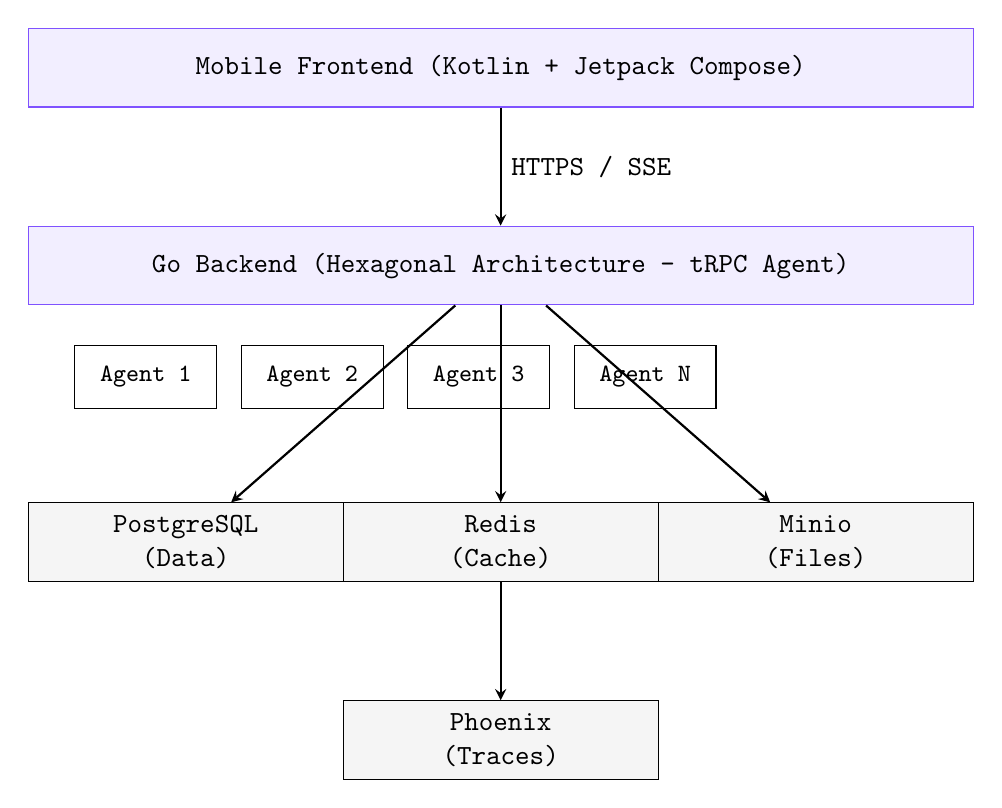
\begin{tikzpicture}[
        node distance=1.5cm,
        box/.style={rectangle, draw, fill=lightgray, minimum width=4cm, minimum height=1cm, align=center},
        purplebox/.style={rectangle, draw=kotlinpurple, fill=kotlinpurple!10, minimum width=4cm, minimum height=1cm, align=center},
        smallbox/.style={rectangle, draw, fill=white, minimum width=1.8cm, minimum height=0.8cm, align=center, font=\small},
        arrow/.style={->, thick, >=stealth}
    ]

        % Frontend
        \node[purplebox, minimum width=12cm] (frontend) {Mobile Frontend (Kotlin + Jetpack Compose)};

        % Backend
        \node[purplebox, minimum width=12cm, below=of frontend] (backend) {Go Backend (Hexagonal Architecture - tRPC Agent)};

        % Agents inside backend
        \node[smallbox, below=0.5cm of backend.south west, xshift=1.5cm] (agent1) {Agent 1};
        \node[smallbox, right=0.3cm of agent1] (agent2) {Agent 2};
        \node[smallbox, right=0.3cm of agent2] (agent3) {Agent 3};
        \node[smallbox, right=0.3cm of agent3] (agentn) {Agent N};

        % Databases
        \node[box, below=2.5cm of backend, xshift=-4cm] (postgres) {PostgreSQL\\(Data)};
        \node[box, below=2.5cm of backend] (redis) {Redis\\(Cache)};
        \node[box, below=2.5cm of backend, xshift=4cm] (minio) {Minio\\(Files)};

        % Phoenix
        \node[box, below=of redis] (phoenix) {Phoenix\\(Traces)};

        % Arrows
        \draw[arrow] (frontend) -- node[right] {HTTPS / SSE} (backend);
        \draw[arrow] (backend) -- (postgres);
        \draw[arrow] (backend) -- (redis);
        \draw[arrow] (backend) -- (minio);
        \draw[arrow] (redis) -- (phoenix);

    \end{tikzpicture}
    \caption{Ora system global architecture}
    \label{fig:architecture}
\end{figure}

% ----------------------------------------------------------------------------
\section{Use Case Diagram}

The use case diagram illustrates the main interactions between users and the Ora application. Users must first authenticate before accessing the core features of the platform. Once authenticated, they can browse available agents, select one to interact with, and engage in conversations.

The chat functionality encompasses sending messages, viewing \gls{streaming} responses in real-time, accessing conversation history, and managing sessions. Profile management allows users to customize their experience through avatar uploads, theme selection, and language preferences.

\begin{figure}[H]
    \centering
    \includegraphics[width=\textwidth]{usecase.png}
    \caption{Use case diagram showing user interactions with the Ora platform}
    \label{fig:usecase}
\end{figure}

% ----------------------------------------------------------------------------
\section{Class Diagram}

The complete class diagram contains over 100 classes spanning all architectural layers. Due to its size, a simplified version focusing on core domain entities is presented below.

\begin{figure}[H]
    \centering
    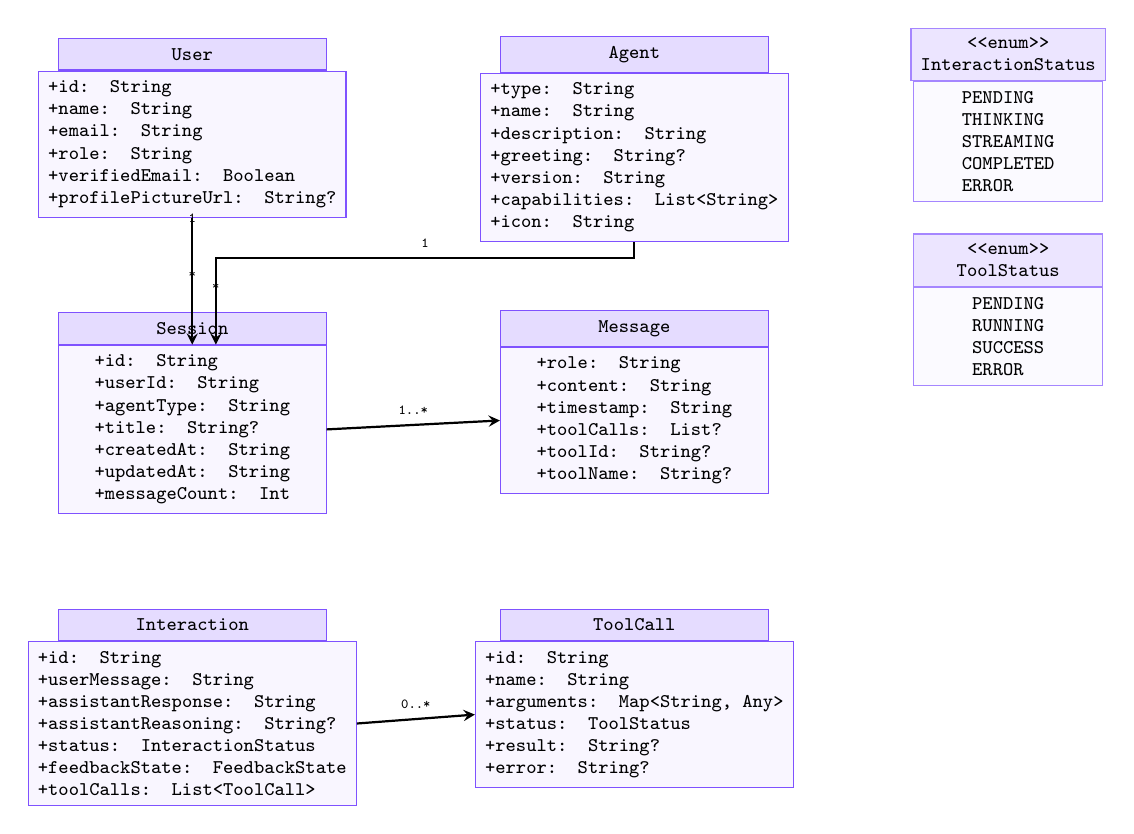
\begin{tikzpicture}[
        node distance=0.6cm and 1.8cm,
        class/.style={rectangle, draw=kotlinpurple, fill=kotlinpurple!5, minimum width=3.4cm, align=left, font=\ttfamily\scriptsize},
        classname/.style={rectangle, draw=kotlinpurple, fill=kotlinpurple!20, minimum width=3.4cm, align=center, font=\ttfamily\scriptsize\bfseries},
        enum/.style={rectangle, draw=kotlinpurple!70, fill=kotlinpurple!3, minimum width=2.4cm, align=left, font=\ttfamily\scriptsize},
        enumname/.style={rectangle, draw=kotlinpurple!70, fill=kotlinpurple!15, minimum width=2.4cm, align=center, font=\ttfamily\scriptsize\bfseries},
        relation/.style={->, thick, >=stealth}
    ]
        % User
        \node[classname] (username) {User};
        \node[class, below=0cm of username] (user) {
            +id: String\\
            +name: String\\
            +email: String\\
            +role: String\\
            +verifiedEmail: Boolean\\
            +profilePictureUrl: String?
        };

        % Agent
        \node[classname, right=2.2cm of username] (agentname) {Agent};
        \node[class, below=0cm of agentname] (agent) {
            +type: String\\
            +name: String\\
            +description: String\\
            +greeting: String?\\
            +version: String\\
            +capabilities: List<String>\\
            +icon: String
        };

        % Session
        \node[classname, below=1.2cm of user] (sessionname) {Session};
        \node[class, below=0cm of sessionname] (session) {
            +id: String\\
            +userId: String\\
            +agentType: String\\
            +title: String?\\
            +createdAt: String\\
            +updatedAt: String\\
            +messageCount: Int
        };

        % Message
        \node[classname, right=2.2cm of sessionname] (msgname) {Message};
        \node[class, below=0cm of msgname] (msg) {
            +role: String\\
            +content: String\\
            +timestamp: String\\
            +toolCalls: List?\\
            +toolId: String?\\
            +toolName: String?
        };

        % Interaction
        \node[classname, below=1.2cm of session] (intname) {Interaction};
        \node[class, below=0cm of intname] (int) {
            +id: String\\
            +userMessage: String\\
            +assistantResponse: String\\
            +assistantReasoning: String?\\
            +status: InteractionStatus\\
            +feedbackState: FeedbackState\\
            +toolCalls: List<ToolCall>
        };

        % ToolCall
        \node[classname, right=2.2cm of intname] (toolname) {ToolCall};
        \node[class, below=0cm of toolname] (tool) {
            +id: String\\
            +name: String\\
            +arguments: Map<String, Any>\\
            +status: ToolStatus\\
            +result: String?\\
            +error: String?
        };

        % Enums on the right
        \node[enumname, right=1.8cm of agentname] (isname) {<<enum>>\\InteractionStatus};
        \node[enum, below=0cm of isname] (is) {
            PENDING\\
            THINKING\\
            STREAMING\\
            COMPLETED\\
            ERROR
        };

        \node[enumname, below=0.4cm of is] (tsname) {<<enum>>\\ToolStatus};
        \node[enum, below=0cm of tsname] (ts) {
            PENDING\\
            RUNNING\\
            SUCCESS\\
            ERROR
        };

        % Relations
        \draw[relation] (user.south) -- ++(0,-0.2) -| node[pos=0.25, above, font=\tiny] {1} node[pos=0.75, above, font=\tiny] {*} (session.north);
        \draw[relation] (agent.south) -- ++(0,-0.2) -| node[pos=0.25, above, font=\tiny] {1} node[pos=0.75, above, font=\tiny] {*} ([xshift=0.3cm]session.north);
        \draw[relation] (session.east) -- node[above, font=\tiny] {1..*} (msg.west);
        \draw[relation] (int.east) -- node[above, font=\tiny] {0..*} (tool.west);

    \end{tikzpicture}
    \caption{Simplified class diagram -- Domain entities}
    \label{fig:classdiagram}
\end{figure}

The domain layer defines the fundamental entities: \texttt{User} represents authenticated users, \texttt{Agent} encapsulates AI agent metadata, \texttt{Session} tracks conversation instances, and \texttt{Message} stores chat messages with optional tool call information.

The \texttt{Interaction} class represents a complete exchange between user and assistant, including any intermediate tool calls. Repository interfaces (\texttt{AuthRepository}, \texttt{AgentRepository}, \texttt{SessionRepository}) define data access contracts following the dependency inversion principle.

The presentation layer implements \gls{mvi} through dedicated ViewModels: \texttt{AuthViewModel}, \texttt{ChatViewModel}, and \texttt{UserProfileViewModel}.

% ----------------------------------------------------------------------------
\section{Screenshots}

\subsection{Authentication}

The authentication screens provide a clean and intuitive interface for user onboarding. The login screen presents email and password fields with the Ora logo prominently displayed, while the registration screen includes additional fields for username and password confirmation. Both screens implement real-time validation, providing immediate feedback when users enter invalid data.

\begin{figure}[H]
    \centering
    \begin{subfigure}[b]{0.45\textwidth}
        \centering
        \includegraphics[width=0.7\textwidth]{login.png}
        \caption{Login screen}
        \label{fig:login}
    \end{subfigure}
    \hfill
    \begin{subfigure}[b]{0.45\textwidth}
        \centering
        \includegraphics[width=0.7\textwidth]{signup.png}
        \caption{Registration screen}
        \label{fig:signup}
    \end{subfigure}
    \caption{Authentication screens with real-time field validation}
    \label{fig:auth-screens}
\end{figure}

\subsection{Home Page and Navigation}

The home screen displays the agent catalog as a collection of cards, each showing the agent's name, description, and icon. Users can browse available agents and select one to begin a conversation. The sidebar navigation drawer provides access to conversation history and allows users to quickly switch between previous sessions or navigate to profile settings.

\begin{figure}[H]
    \centering
    \begin{subfigure}[b]{0.45\textwidth}
        \centering
        \includegraphics[width=0.7\textwidth]{home.png}
        \caption{Agent catalog}
        \label{fig:home}
    \end{subfigure}
    \hfill
    \begin{subfigure}[b]{0.45\textwidth}
        \centering
        \includegraphics[width=0.7\textwidth]{sidebar.png}
        \caption{Side menu (drawer)}
        \label{fig:sidebar}
    \end{subfigure}
    \caption{Main application navigation}
    \label{fig:nav-screens}
\end{figure}

\subsection{Chat Interface}

The chat interface is the core feature of the Ora application. The message input area at the bottom of the screen provides a text field with a send button, optimized for quick and intuitive message composition. User messages appear on the right side of the conversation view, while agent responses are displayed on the left.

The application supports full Markdown rendering including syntax highlighting for code blocks. This is particularly important for technical agents that may provide code examples or technical documentation in their responses.

\begin{figure}[H]
    \centering
    \begin{subfigure}[b]{0.45\textwidth}
        \centering
        \includegraphics[width=0.7\textwidth]{input.png}
        \caption{Message input area}
        \label{fig:input}
    \end{subfigure}
    \hfill
    \begin{subfigure}[b]{0.45\textwidth}
        \centering
        \includegraphics[width=0.7\textwidth]{chat.png}
        \caption{Conversation with agent}
        \label{fig:chat}
    \end{subfigure}
    \caption{Chat interface with Markdown rendering and syntax highlighting}
    \label{fig:chat-screens}
\end{figure}

During request processing, the application displays a thinking indicator that informs users the agent is analyzing their message. This visual feedback is essential for maintaining a responsive feel even when complex reasoning operations are being performed on the backend.

\begin{figure}[H]
    \centering
    \includegraphics[width=0.4\textwidth]{reflexion.png}
    \caption{Thinking indicator during request processing}
    \label{fig:reflexion}
\end{figure}

\subsection{Tool Calls}

One of the distinguishing features of Ora is its support for agent tool calls. When an agent needs to perform actions such as searching for information, executing code, or accessing external services, these operations are displayed transparently to the user.

The tool call interface shows which tools are being invoked along with their parameters, allowing users to understand exactly what actions the agent is taking on their behalf. Once tool execution completes, the results are integrated into the conversation flow alongside the agent's final response.

\begin{figure}[H]
    \centering
    \begin{subfigure}[b]{0.45\textwidth}
        \centering
        \includegraphics[width=0.7\textwidth]{tools.png}
        \caption{Tool execution}
        \label{fig:tools}
    \end{subfigure}
    \hfill
    \begin{subfigure}[b]{0.45\textwidth}
        \centering
        \includegraphics[width=0.7\textwidth]{tools+answer.png}
        \caption{Result with response}
        \label{fig:tools-answer}
    \end{subfigure}
    \caption{Display of tool calls made by the agent}
    \label{fig:tools-screens}
\end{figure}

\subsection{User Profile}

The user profile screen centralizes all account management and preference settings. Users can view and edit their personal information, upload a custom profile picture, and customize the application experience through theme and language selection. Account actions including logout and account deletion are also accessible from this screen.

\begin{figure}[H]
    \centering
    \includegraphics[width=0.4\textwidth]{user.png}
    \caption{Profile page with settings (theme, language, account)}
    \label{fig:user}
\end{figure}

% ----------------------------------------------------------------------------
\section{Technical Challenges Overcome}

The development of Ora presented several significant technical challenges that required careful consideration and innovative solutions. These challenges primarily arose from the need to provide a seamless real-time chat experience while maintaining clean architecture principles.

\subsection{Real-time SSE Streaming}

The most complex challenge involved implementing \gls{sse} \gls{streaming} for AI responses. Unlike traditional HTTP requests that return complete responses, \gls{sse} requires maintaining a persistent connection and processing data as it arrives token by token.

The Android lifecycle adds additional complexity, as connections must survive configuration changes like screen rotations while being properly cleaned up when the activity is destroyed. Events arrive on IO threads and must be dispatched to the main thread for UI updates without blocking the interface during rapid event bursts.

The solution implements a buffering mechanism with implicit debouncing, combined with Kotlin \gls{flow} operators like \texttt{conflate()} to handle backpressure when events arrive faster than the UI can process them.

\subsection{Custom Markdown Rendering}

Jetpack Compose does not provide a native Markdown component, requiring a hybrid approach using the Markwon library within an \texttt{AndroidView}. This creates interoperability challenges between the Compose theming system and traditional Android Views.

Syntax highlighting for code blocks across 13 programming languages was implemented through a custom \texttt{SyntaxHighlighter} with regex-based parsing. To address performance concerns with large code blocks, the solution employs lazy parsing and an LRU cache to memoize results.

\subsection{MVI Architecture with Streaming State}

The standard \gls{mvi} pattern assumes discrete states with atomic transitions, but \gls{streaming} introduces a continuously evolving state that updates multiple times per second. The solution uses composite states with independent sub-states, allowing the streaming content to be updated without triggering unnecessary recomposition of unrelated UI elements.

\begin{table}[H]
    \centering
    \begin{tabularx}{\textwidth}{|l|c|X|}
        \hline
        \rowcolor{lightgray}
        \textbf{Challenge} & \textbf{Complexity} & \textbf{Solution} \\
        \hline
        Real-time \gls{sse} \gls{streaming} & High & Buffering with debounce, StateFlow with conflate \\
        \hline
        Custom Markdown rendering & High & Markwon + custom SyntaxHighlighter with LRU cache \\
        \hline
        \gls{mvi} architecture streaming & Medium & Composite states with independent sub-states \\
        \hline
        Auth with refresh token & Medium & AuthInterceptor with Mutex to avoid race conditions \\
        \hline
        OkHttp/Ktor integration & Medium & Shared Hilt module, common factory \\
        \hline
    \end{tabularx}
    \caption{Summary of major technical challenges}
    \label{tab:challenges}
\end{table}



% Technical Specifications
% ============================================================================
% PART II: TECHNICAL SPECIFICATIONS
% ============================================================================

\chapter{Technical Specifications}

\section{Architecture}

\subsection{Clean Architecture}

Ora follows Clean Architecture principles to ensure separation of concerns, testability, and maintainability. The codebase is organized into four distinct layers, each with clear responsibilities and dependencies flowing inward.

\begin{figure}[H]
    \centering
    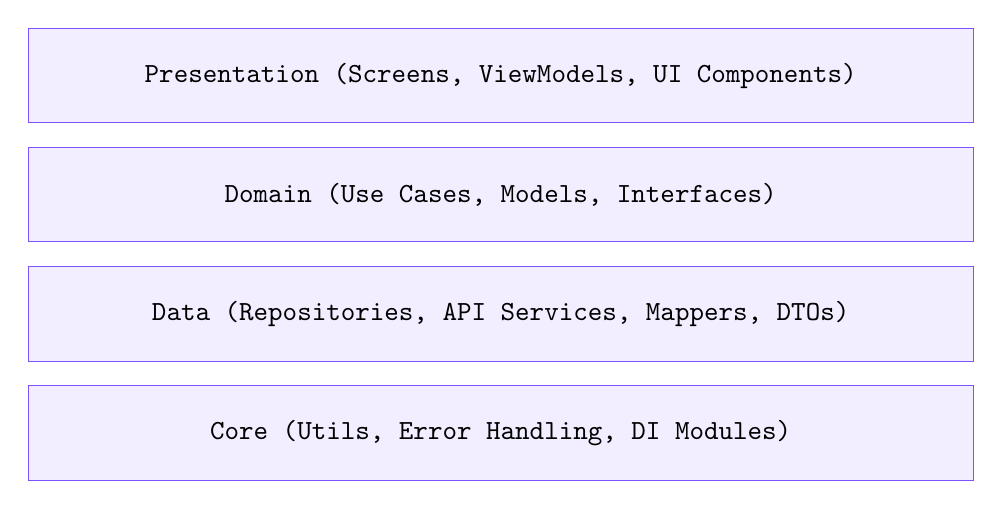
\begin{tikzpicture}[
        node distance=0.3cm,
        layer/.style={rectangle, draw=kotlinpurple, fill=kotlinpurple!10, minimum width=12cm, minimum height=1.2cm, align=center}
    ]
        \node[layer] (pres) {Presentation (Screens, ViewModels, UI Components)};
        \node[layer, below=of pres] (domain) {Domain (Use Cases, Models, Interfaces)};
        \node[layer, below=of domain] (data) {Data (Repositories, API Services, Mappers, DTOs)};
        \node[layer, below=of data] (core) {Core (Utils, Error Handling, DI Modules)};
    \end{tikzpicture}
    \caption{Clean Architecture layers in Ora}
    \label{fig:clean-arch}
\end{figure}

The \textbf{Core Layer} contains utilities, constants, error handling mechanisms, and dependency injection modules. This layer has no dependencies on other layers and provides foundational components used throughout the application.

The \textbf{Data Layer} implements the repository interfaces defined in the domain layer. It handles all external data operations including API calls, local storage, and data mapping. DTOs are converted to domain models through dedicated mapper classes, ensuring the domain layer remains independent of external data representations.

The \textbf{Domain Layer} represents the business logic of the application. It defines the core models (User, Agent, Session, Message), repository interfaces, and use cases. This layer is completely independent of frameworks and external libraries, making it highly testable and portable.

The \textbf{Presentation Layer} handles all UI-related concerns using Jetpack Compose. ViewModels manage UI state and coordinate with use cases to perform business operations. The layer implements the MVI pattern for predictable state management.

\subsection{MVI Pattern}

The application uses the Model-View-Intent (MVI) pattern for state management in the presentation layer.

\subsubsection{Why MVI over MVVM?}

MVI was chosen over MVVM for several technical reasons specific to Ora's requirements.

The first consideration is \textbf{unidirectional data flow}. In a chat application with real-time streaming, predictable state changes are critical. MVI enforces a single direction: Intent → Model → View, eliminating ambiguity about how and when state changes occur. MVVM's bidirectional binding can lead to unpredictable state updates when handling rapid SSE events.

The second reason is \textbf{state immutability}. MVI uses immutable state objects, making it trivial to compare previous and current states. This is essential for optimizing Compose recomposition during streaming, where content updates multiple times per second.

The third advantage is \textbf{debugging and reproducibility}. Every state transition in MVI is triggered by an explicit Intent. This creates a clear audit trail, making it easier to debug issues in complex flows like tool call sequences or authentication refreshes.

\begin{figure}[H]
    \centering
    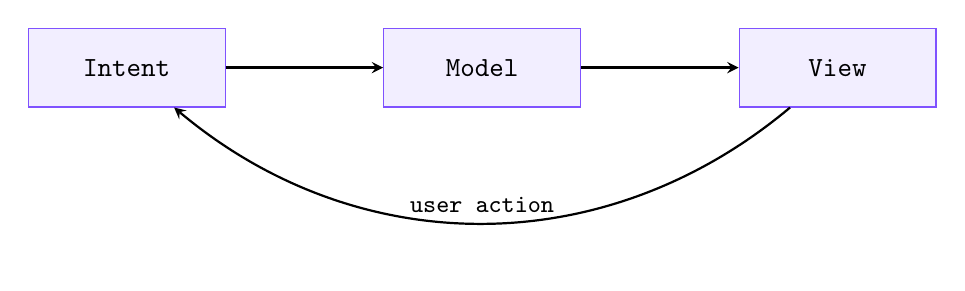
\begin{tikzpicture}[
        node distance=2cm,
        box/.style={rectangle, draw=kotlinpurple, fill=kotlinpurple!10, minimum width=2.5cm, minimum height=1cm, align=center},
        arrow/.style={->, thick, >=stealth}
    ]
        \node[box] (intent) {Intent};
        \node[box, right=of intent] (model) {Model};
        \node[box, right=of model] (view) {View};

        \draw[arrow] (intent) -- (model);
        \draw[arrow] (model) -- (view);
        \draw[arrow, bend left=40] (view) to node[above] {\small user action} (intent);
    \end{tikzpicture}
    \caption{MVI unidirectional data flow}
    \label{fig:mvi}
\end{figure}

% ----------------------------------------------------------------------------
\section{API Interaction}

\subsection{Authentication Endpoints}

\begin{table}[H]
    \centering
    \begin{tabularx}{\textwidth}{|l|l|X|X|}
        \hline
        \rowcolor{lightgray}
        \textbf{Endpoint} & \textbf{Method} & \textbf{Description} & \textbf{Returns} \\
        \hline
        /auth/login & POST & Authenticates user with email/password & User + token \\
        \hline
        /auth/register & POST & Creates new user account & User + token \\
        \hline
        /auth/logout & POST & Invalidates current session & Status \\
        \hline
        /auth/refresh & POST & Refreshes expired access token & New token \\
        \hline
        /auth/me & GET & Retrieves current user info & User profile \\
        \hline
        /auth/me & DELETE & Deletes user account & Status \\
        \hline
        /auth/me/profile-picture & POST & Uploads profile picture & Picture URL \\
        \hline
    \end{tabularx}
    \caption{Authentication API endpoints}
    \label{tab:auth-api}
\end{table}

\subsection{Agent Endpoints}

\begin{table}[H]
    \centering
    \begin{tabularx}{\textwidth}{|l|l|X|X|}
        \hline
        \rowcolor{lightgray}
        \textbf{Endpoint} & \textbf{Method} & \textbf{Description} & \textbf{Returns} \\
        \hline
        /agents & GET & Lists all available agents & Agent array \\
        \hline
        /agents/\{type\} & GET & Gets specific agent info & Agent details \\
        \hline
    \end{tabularx}
    \caption{Agent API endpoints}
    \label{tab:agent-api}
\end{table}

\subsection{Session Endpoints}

\begin{table}[H]
    \centering
    \begin{tabularx}{\textwidth}{|l|l|X|X|}
        \hline
        \rowcolor{lightgray}
        \textbf{Endpoint} & \textbf{Method} & \textbf{Description} & \textbf{Returns} \\
        \hline
        /agents/\{type\}/sessions & GET & Lists user sessions & Session array \\
        \hline
        /agents/\{type\}/sessions & POST & Creates new session & Session ID \\
        \hline
        /agents/\{type\}/sessions/\{id\} & GET & Gets session + history & Messages \\
        \hline
        /agents/\{type\}/sessions/\{id\} & DELETE & Deletes session & Status \\
        \hline
        /agents/\{type\}/sessions/\{id\}/message & POST & Sends message & Stream ID \\
        \hline
    \end{tabularx}
    \caption{Session API endpoints}
    \label{tab:session-api}
\end{table}

% ----------------------------------------------------------------------------
\section{SSE Streaming}

\subsection{Overview}

Server-Sent Events (\gls{sse}) is used for real-time streaming of AI responses. Unlike WebSockets, SSE provides a simpler unidirectional protocol perfectly suited for the chat use case where only the server needs to push data to the client.

\subsection{Connection Flow}

The streaming process follows a specific sequence:

\begin{enumerate}
    \item Client sends message via POST to /agents/\{type\}/sessions/\{id\}/message
    \item Server returns a stream ID
    \item Client opens SSE connection to /stream/\{streamId\}
    \item Server pushes events as AI generates response
    \item Connection closes on "done" or "close" event
\end{enumerate}

\subsection{Event Types}

\begin{table}[H]
    \centering
    \begin{tabularx}{\textwidth}{|l|X|}
        \hline
        \rowcolor{lightgray}
        \textbf{Event} & \textbf{Description} \\
        \hline
        delta & Incremental content token (streaming mode enabled) \\
        \hline
        message & Complete message in one block (streaming mode disabled) \\
        \hline
        reasoning & AI reasoning/thinking content \\
        \hline
        tool\_call & Agent initiating tool execution \\
        \hline
        tool\_response & Result from tool execution \\
        \hline
        thinking\_start & AI begins reasoning phase \\
        \hline
        thinking\_end & AI completes reasoning phase \\
        \hline
        error & Error during processing \\
        \hline
        done & Stream completed successfully \\
        \hline
        close & Connection should be closed \\
        \hline
        heartbeat & Keep-alive signal \\
        \hline
    \end{tabularx}
    \caption{SSE event types}
    \label{tab:sse-events}
\end{table}

\subsection{Implementation}

SSE is implemented using OkHttp's EventSource client rather than Ktor, as Ktor does not natively support SSE. The \texttt{SSEClient} class manages connection lifecycle, event parsing, and error handling. Events are parsed by \texttt{SSEEventMapper} and converted to sealed \texttt{StreamEvent} classes, enabling type-safe handling in the ViewModel.

% ----------------------------------------------------------------------------
\section{Markdown Rendering}

\subsection{Architecture}

Markdown rendering combines the Markwon library with custom syntax highlighting. Since Jetpack Compose lacks native Markdown support, rendering is performed in an \texttt{AndroidView} wrapper containing a \texttt{TextView}.

\subsection{Components}

\textbf{MarkdownText} is a Composable wrapper that creates and configures the Markwon instance, handles theme changes, and bridges Compose with Android Views.

\textbf{CodeBlock} is a custom component for displaying code blocks with syntax highlighting, language label, and copy-to-clipboard functionality.

\textbf{SyntaxHighlighter} is a custom regex-based highlighter supporting 13 languages. While Prism4j is available in dependencies, a custom implementation was chosen to avoid annotation processing complexity and provide finer control over the Gruvbox color scheme.

\subsection{Supported Languages}

Kotlin, Java, Python, JavaScript, TypeScript, Go, Rust, C, C++, Swift, SQL, JSON, XML/HTML.

% ----------------------------------------------------------------------------
\section{Libraries}

\begin{table}[H]
    \centering
    \begin{tabularx}{\textwidth}{|l|l|X|}
        \hline
        \rowcolor{lightgray}
        \textbf{Library} & \textbf{Version} & \textbf{Purpose} \\
        \hline
        Ktor Client & 3.0.2 & HTTP client for REST API (Kotlin-first, coroutines) \\
        \hline
        OkHttp SSE & 4.12.0 & SSE client for real-time streaming \\
        \hline
        Hilt & 2.58 & Dependency injection (compile-time, ViewModels) \\
        \hline
        Kotlinx Serialization & 1.7.3 & JSON serialization (no reflection, type-safe) \\
        \hline
        Jetpack Compose & BOM 2025.01.00 & Declarative UI framework \\
        \hline
        DataStore & 1.1.1 & Preferences storage (coroutines, type-safe) \\
        \hline
        Security Crypto & 1.1.0-alpha06 & Encrypted token storage (Keystore) \\
        \hline
        Coil & 3.0.4 & Image loading (Compose-native, Ktor) \\
        \hline
        Markwon & 4.6.2 & Markdown rendering (extensible, tables) \\
        \hline
        Coroutines & 1.9.0 & Async programming (Flow, structured) \\
        \hline
    \end{tabularx}
    \caption{Main libraries and their purposes}
    \label{tab:libraries}
\end{table}

\subsection{Library Selection Criteria}

Each library was selected based on the following criteria:

\textbf{Kotlin-first}: Native Kotlin API without Java wrappers, leveraging language features like coroutines, sealed classes, and extension functions.

\textbf{Coroutine support}: Native integration with suspend functions and Flow for reactive programming.

\textbf{Maintenance}: Active development, regular updates, and strong community support.

\textbf{Performance}: Minimal impact on APK size and runtime performance.

% ----------------------------------------------------------------------------
\section{Testing}

\subsection{Testing Strategy}

The application follows a comprehensive testing strategy organized in four tiers based on criticality:

\begin{itemize}
    \item \textbf{Tier 1 - Critical:} Security-sensitive components and complex parsing logic (SSE events, session reconstruction, authentication interceptor)
    \item \textbf{Tier 2 - High Priority:} Business logic in use cases that orchestrate application behavior
    \item \textbf{Tier 3 - Medium Priority:} Data layer components including mappers and repository implementations
    \item \textbf{Tier 4 - Lower Priority:} Presentation layer ViewModels with UI state management
\end{itemize}

\subsection{Test Libraries}

\begin{table}[H]
    \centering
    \begin{tabularx}{\textwidth}{|l|l|X|}
        \hline
        \rowcolor{lightgray}
        \textbf{Library} & \textbf{Version} & \textbf{Purpose} \\
        \hline
        JUnit & 4.13.2 & Test framework \\
        \hline
        MockK & 1.13.10 & Kotlin mocking library \\
        \hline
        Truth & 1.4.2 & Fluent assertions \\
        \hline
        Turbine & 1.1.0 & Flow testing utilities \\
        \hline
        Coroutines Test & 1.9.0 & Coroutine testing \\
        \hline
    \end{tabularx}
    \caption{Testing libraries}
    \label{tab:test-libs}
\end{table}

\subsection{Test Coverage}

\begin{table}[H]
    \centering
    \begin{tabularx}{\textwidth}{|l|X|l|l|}
        \hline
        \rowcolor{lightgray}
        \textbf{Layer} & \textbf{Components} & \textbf{Test Files} & \textbf{Tests} \\
        \hline
        Core & Utils, Error Mapping, Network & 4 & 30 \\
        \hline
        Domain & Use Cases, Models & 14 & 72 \\
        \hline
        Data & Mappers, Repository & 5 & 69 \\
        \hline
        Presentation & ViewModels & 3 & 48 \\
        \hline
        \textbf{Total} & - & \textbf{26} & \textbf{219} \\
        \hline
    \end{tabularx}
    \caption{Test coverage by layer}
    \label{tab:test-coverage}
\end{table}

\subsection{Test Structure}

Tests are organized mirroring the source code structure, ensuring clear correspondence between implementation and tests:

\begin{itemize}
    \item \texttt{core/} -- ResultTest, DateTimeUtilTest, ErrorMapperTest, AuthInterceptorTest
    \item \texttt{data/mapper/} -- SSEEventMapperTest, SessionMapperTest, UserMapperTest, AgentMapperTest
    \item \texttt{data/repository/} -- AuthRepositoryImplTest
    \item \texttt{domain/model/} -- SessionInteractionsTest
    \item \texttt{domain/usecase/auth/} -- Login, Register, GetCurrentUser, Logout, DeleteAccount, UploadProfilePicture
    \item \texttt{domain/usecase/agent/} -- GetAgentsUseCaseTest
    \item \texttt{domain/usecase/session/} -- GetSessions, CreateSession, DeleteSession, GetSessionHistory, SendMessage, StreamResponse
    \item \texttt{presentation/features/} -- AuthViewModelTest, ChatViewModelTest, UserProfileViewModelTest
\end{itemize}

\subsection{Critical Tests}

\textbf{SSEEventMapperTest} (39 tests) validates parsing of all 13+ SSE event types including delta content accumulation, tool call/response structures, error handling with codes, and graceful degradation for malformed JSON.

\textbf{SessionInteractionsTest} (15 tests) tests the complex algorithm that reconstructs user-assistant interaction pairs from raw message history, including tool call matching, pending status detection, and metadata conversion.

\textbf{AuthInterceptorTest} (12 tests) verifies token injection for authenticated requests, public endpoint bypassing, 401 response handling, and concurrent refresh prevention using atomic flags.

\subsection{Testing Patterns}

\textbf{Use Case Tests:} Each use case is tested with mocked repository dependencies. Tests verify input validation, successful execution paths, error propagation, and correct repository method invocation.

\textbf{ViewModel Tests:} ViewModels are tested using \texttt{UnconfinedTestDispatcher} for synchronous execution. Turbine is used to test Flow emissions (effects) such as navigation events and toasts.

\textbf{Mapper Tests:} Data mappers are tested to ensure correct field mapping between DTOs and domain models, with special attention to nullable fields and nested objects.

% ----------------------------------------------------------------------------
\section{Future Evolution}

The Ora platform has been designed with extensibility in mind, and several enhancements are planned for future development phases. This section presents the two major features on the roadmap along with additional improvements.

\subsection{Multimodal Support}

The current architecture already supports multimodal interactions at the backend level, with existing endpoints for attachment uploads that are not yet integrated into the mobile application. The next major release will enable users to enrich their conversations with images, documents, and audio content.

Users will be able to attach images directly to their messages, providing visual context that agents can analyze and reference in their responses. Document support will include PDF, Word, and plain text formats, allowing users to share technical documentation or reference materials during conversations. Voice input through audio recording will offer an alternative interaction mode, with server-side transcription converting speech to text before processing.

From a technical perspective, this feature requires implementing an \texttt{AttachmentRepository} to handle file upload and download operations, adding multipart form data support to the Ktor client, and creating new UI components for attachment selection and preview. File compression and validation will ensure optimal performance and security.

\subsection{Knowledge Base Management}

One of the most powerful upcoming features is the exposure of the vector knowledge base to end users. The backend already maintains a dedicated vector database for each agent and user, enabling contextual retrieval during conversations. Future versions will provide a complete interface for users to manage their personal knowledge base.

Users will be able to upload documents that become part of their personal context, viewable and searchable through an in-app browser. When agents reference information from the knowledge base during responses, the interface will display which documents contributed to the answer, providing transparency into the retrieval process. Bulk import and export operations will facilitate migration and backup of knowledge bases.

\begin{table}[H]
    \centering
    \begin{tabularx}{\textwidth}{|l|l|X|}
        \hline
        \rowcolor{lightgray}
        \textbf{Method} & \textbf{Endpoint} & \textbf{Description} \\
        \hline
        GET & /knowledge/documents & List all documents in user's knowledge base \\
        \hline
        POST & /knowledge/documents & Upload a new document \\
        \hline
        GET & /knowledge/documents/\{id\} & Retrieve document content and metadata \\
        \hline
        DELETE & /knowledge/documents/\{id\} & Remove document from knowledge base \\
        \hline
        GET & /knowledge/search & Search documents by semantic similarity \\
        \hline
    \end{tabularx}
    \caption{Planned knowledge base API endpoints}
    \label{tab:kb-endpoints}
\end{table}

The implementation will leverage the existing server-side embedding pipeline for vector generation. Document chunking strategies will need to balance retrieval precision with context coherence. Preview rendering will require format-specific handlers, such as PDF.js for PDF documents and the existing Markwon renderer for markdown files. Storage quotas and document size limits will be defined to ensure fair resource allocation.

\subsection{Additional Improvements}

Beyond these major features, several quality-of-life improvements are planned. Offline mode will cache recent conversations locally using Room database, allowing users to browse their history without network connectivity. Push notifications will alert users when agents complete long-running tasks or when collaborative sessions receive new messages.

Collaborative sessions will enable users to share conversations with colleagues, facilitating team workflows around AI interactions. Agent customization will allow power users to define custom system prompts and adjust model parameters for specific use cases. Finally, an analytics dashboard will provide insights into usage patterns, helping users understand their interaction history and optimize their workflows.


% ----------------------------------------------------------------------------
% APPENDICES
% ----------------------------------------------------------------------------
\appendix

% Glossary
\printglossaries

\end{document}
